\documentclass[twocolumn,fleqn,a4paper,10pt]{jarticle}
\usepackage{amsmath,amssymb}
\usepackage[dvipdfmx]{graphicx}
\usepackage{emathP}

\title{微分積分I夏課題} 
\date{\today} 

\hoffset = -40pt
\voffset = -110pt
\textwidth = 180mm
\textheight = 275mm

\begin{document}
\setlength{\parindent}{0pt}
\setlength{\columnseprule}{0.4pt}

\renewcommand{\thesection}{\fbox{\arabic{section}}}
\renewcommand{\labelenumi}{(\theenumi)}

\maketitle

%1
\section{}
\begin{enumerate}
\item \begin{flalign*}
	y\phantom{`}&=(x^2+2x)(3x+1)\\
	y'&=(2x+2)(3x+1)+(x^2+2x)(3)\\ 
	&=6x^2+8x+2+3x^2+6x\\
	&=9x^2+14x+2
\end{flalign*}
\item \begin{flalign*}
	y&=(2x^3+6x)(7x-5)\\
	y'&=(6x^2+6)(7x-5)+(2x^3+6x)(7)\\
	&=42x^3-30x^2+42x-30+14x^3+42x\\
	&=56x^3-30x^2+84x-30
\end{flalign*}
\item \begin{flalign*}
	y&=(x+1)(x^2-4x-5)\\
	y'&=1(x^2-4x-5)+(x+1)(2x-4)\\
	&=x^2-4x-5+2x^2-2x-4\\
	&=3x^2-6x-9
\end{flalign*}
\item \begin{flalign*}
	y&=(x-1)(x-2)(x-3)\\
	y'&=1(x-2)(x-3)+1(x-1)(x-3)\\
	&\qquad+1(x-1)(x-2)\\
	&=x^2-5x+6+x^2-4x+3+x^2-3x+2\\
	&=3x^2-12x+11
\end{flalign*}
\end{enumerate}

%2
\section{}
\begin{enumerate}
\item\begin{flalign*}
	y&=\frac{2x-3}{3x+1}\\
	y'&=\frac{(2)(3x+1)-(2x-3)(3)}{(3x+1)^2}\\
	&=\frac{6x+2-6x+9}{(3x+1)^2}\\
	&=\frac{11}{(3x+1)^2}
\end{flalign*}
\item \begin{flalign*}
	y&=\frac{x^2-1}{3x^2+1}\\
	y'&=\frac{(2x)(3x^2+1)-(x^2-1)(6x)}{(3x^2+1)^2}\\
	&=\frac{6x^3+2x-6x^3+6x}{(3x^2+1)^2}\\
	&=\frac{8x}{(3x^2+1)^2}
\end{flalign*}
\item \begin{flalign*}
	y&=\frac{1}{2x-3}\\
	y'&=-\frac{2}{(2x-3)^2}
\end{flalign*}
\item \begin{flalign*}
	y&=\frac{x+1}{x^2+2x+2}\\
	y'&=\frac{(1)(x^2+2x+2)-(x+1)(2x+2)}{(x^2+2x+2)^2}\\
	&=\frac{x^2+2x+2-2x^2-4x-2}{(x^2+2x+2)^2}\\
	&=\frac{-x^2-2x}{(x^2+2x+2)^2}\\
	&=-\frac{x(x+2)}{(x^2+2x+2)^2}
\end{flalign*}
\end{enumerate}

%3
\section{}
\begin{enumerate}
\item \begin{flalign*}
	y&=\frac{1}{x^2}\\
	y'&=-\frac{2x}{x^4}\\
	&=-\frac{2}{x^3}
\end{flalign*}
\item \begin{flalign*}
	y&=\frac{3}{x}-\frac{2}{x^3}\\
	y'&=-\frac{3}{x^2}+\frac{6x^2}{x^4}
\end {flalign*}
\item \begin{flalign*}
	y&=(1-x^2)(1+\frac{1}{x^2})\\
	y'&=(-2x)(1+\frac{1}{x^2})+(1-x^2)(-\frac{2}{x^3})\\
	&=-2x-\frac{2}{x}-\frac{2}{x^3}+\frac{2}{x}\\
	&=-2x-\frac{2}{x^3}
\end {flalign*}
\item \begin{flalign*}
	y&=(2x-3)^3\\
	y'&=3(2x-3)^2(2)\\
	&=6(2x-3)^2
\end {flalign*}
\item \begin{flalign*}
	y&=(x^2+1)^4\\
	y'&=4(x^2+1)^3(2x)\\
	&=8x(x^2+1)^3\\
\end {flalign*}
\item \begin{flalign*}
	y&=(3x^2-4x+1)^2\\
	y'&=2(3x^2-4x+1)(6x-4)\\
	&=4(3x-2)(3x^2-4x+1)
\end {flalign*}
\item \begin{flalign*}
	y&=\frac{1}{(3-4x)^2}\\
	y'&=-\frac{2(3-4x)(-4)}{(3-4x)^4}\\
	&=\frac{8(3-4x)}{(3-4x)^4}\\
	&=\frac{8}{(3-4x)^3}
\end {flalign*}
\item \begin{flalign*}
	y&=\frac{1}{(x^2-1)^4}\\
	y'&=-\frac{4(x^2-1)^3(2x)}{(x^2-1)^8}\\
	&=-\frac{8x(x^2-1)^3}{(x^2-1)^8}\\
	&=-\frac{8x}{(x^2-1)^5}
\end {flalign*}
\end{enumerate}

%4
\section{}
\begin{enumerate}
\item \begin{flalign*}
	y&=\sqrt[3]{x^2}\\
	y'&=\frac{2}{3}\sqrt[3]x
\end{flalign*}
\item \begin{flalign*}
	y&=\sqrt{3x+1}\\
	y'&=\frac{1}{2}(3x+1)^{-\frac{1}{2}}(3)\\
	&=\frac{3}{2\sqrt{3x+1}}
\end {flalign*}
\item \begin{flalign*}
	y&=\sqrt[3]{x+3}\\
	y'&=\frac{1}{3\sqrt[3]{(x+3)^2}}\\
\end {flalign*}
\item \begin{flalign*}
	y&=\sqrt{x^2+2}\\
	y'&=\frac{2x}{2\sqrt{x^2+2}}\\
	&=\frac{x}{\sqrt{x^2+2}}
\end {flalign*}
\item \begin{flalign*}
	y&=\frac{\sqrt{x}}{x+1}\\
	y'&=\frac{\frac{1}{2\sqrt{x}}(x+1)-\sqrt{x}(1)}{(x+1)^2}\\
	&=\frac{x+1-2x}{2\sqrt{x}(x+1)^2}\\
	&=\frac{1-x}{2\sqrt{x}(x+1)^2}
\end {flalign*}
\item \begin{flalign*}
	y&=\frac{1}{\sqrt{2x+1}}\\
	y'&=-\frac{\frac{2}{2\sqrt{2x+1}}}{2x+1}\\
	&=-\frac{1}{\sqrt{2x+1}(2x+1)}
\end {flalign*}
\end{enumerate}

%5
\section{}
\begin{enumerate}
\item \begin{flalign*}
	y&=x^2(2x+3)^2\\
	y'&=2x(2x+3)^2+(x^2)2(2x+3)(2)\\
	&=2x(2x+3)(2x+3+2x)\\
	&=2x(2x+3)(4x+3)
\end{flalign*}
\item \begin{flalign*}
	y&=(x-1)^2(2x+1)^3\\
	y'&=2(x-1)(2x+1)^3+(x-1)^2 3(2x+1)^2(2)\\
	&=(x-1)(2x+1)^2(2(2x+1)+6(x-1))\\
	&=(x-1)(2x+1)^2(10x-4)\\
	&=2(x-1)(2x+1)^2(5x-2)
\end {flalign*}
\item \begin{flalign*}
	y&=\frac{(4+x^2)^2}{4-x^2}\\
	y'&=\frac{2(4+x^2)(2x)(4-x^2)-(4+x^2)^2(-2x)}{(4-x^2)^2}\\
	&=\frac{2x(4+x^2)(2(4-x^2)+(4+x^2))}{(4-x^2)^2}\\
	&=\frac{2x(4+x^2)(8-2x^2+4+x^2)}{(4-x^2)^2}\\
	&=\frac{2x(4+x^2)(-x^2+12)}{(4-x^2)^2}
\end {flalign*}
\item \begin{flalign*}
	y&=\frac{(2x+1)^3}{(x^2-3)^2}\\
	y'&=\frac{1}{(x^2-3)^2}\{3(2x+1)^2(2)(x^2-3)^2\\
	&\qquad-(2x+1)^3 2(x^2-3)(2x)\}\\
	&=\frac{6(2x+1)^2(x^2-3)^2-4x(2x+1)^3(x^2-3)}{(x^2-3)^4}\\
	&=\frac{2(2x+1)^2(3(x^2-3)-2x(2x+1))}{(x^2-3)^3}\\
	&=\frac{2(2x+1)^2(3x^2-9-4x^2-2x)}{(x^2-3)^3}\\
	&=-\frac{2(2x+1)^2(x^2+2x+9)}{(x^2-3)^3}
\end {flalign*}
\end{enumerate}

%6
\section{}
\begin{enumerate}
\item \begin{flalign*}
	y&=\sqrt{2x+1}\\
	y'&=\frac{2}{2\sqrt{2x+1}}\\
	&=\frac{1}{\sqrt{2x+1}}
\end{flalign*}
\item \begin{flalign*}
	y&=\frac{1+x^2}{\sqrt{x}}\\
	y'&=\frac{2x\sqrt{x}-(1+x^2)\frac{1}{2\sqrt{x}}}{x}\\
	&=\frac{4x^2-(1+x^2)}{2x\sqrt{x}}\\
	&=\frac{3x^2-1}{2x\sqrt{x}}
\end {flalign*}
\item \begin{flalign*}
	y&=\sqrt{x^2+3x+5}\\
	y'&=\frac{2x+3}{2\sqrt{x^2+3x+5}}\\
\end {flalign*}
\item \begin{flalign*}
	y&=\frac{1}{\sqrt{x^2+2x+2}}\\
	y'&=-\frac{\frac{2x+2}{2\sqrt{x^2+2x+2}}}{x^2+2x+2}\\
	&=\frac{x+1}{(x^2+2x+2)\sqrt{x^2+2x+2}}
\end {flalign*}
\end{enumerate}

%7
\section{}
\begin{enumerate}
\item \begin{flalign*}
	y&=\log{(2x-3)}\\
	y'&=\frac{2}{2x-3}
\end{flalign*}
\item \begin{flalign*}
	y&=log(x^2+2x+2)\\
	y'&=\frac{2x+2}{x^2+2x+2}
\end {flalign*}
\item \begin{flalign*}
	y&=\log{\sqrt{1-x^2}}\\
	y'&=\frac{\frac{-2x}{2\sqrt1-x^2}}{\sqrt{1-x^2}}\\
	&=\frac{x}{x^2-1}
\end {flalign*}
\item \begin{flalign*}
	y&=x^2\log{x}\\
	y'&=2x\log{x}+x^2\frac{1}{x}\\
	&=2x\log{x}+x
\end {flalign*}
\item \begin{flalign*}
	y&=\frac{1}{x+log{x}}\\
	y'&=-\frac{1+\frac{1}{x}}{(x+\log{x})^2}\\
	&=-\frac{x+1}{x(x+\log{x})^2}
\end {flalign*}
\item \begin{flalign*}
	y&=x\log{(x^2+1)}\\
	y'&=\log{(x^2+1)}+\frac{2x^2}{x^2+1}
\end {flalign*}
\end{enumerate}

%8
\section{}
\begin{enumerate}
\item \begin{flalign*}
	y&=e^{2x}\\
	y'&=2e^{2x}
\end{flalign*}
\item \begin{flalign*}
	y&=e^{2-3x}\\
	y'&=-3e^{2-3x}\\
\end {flalign*}
\item \begin{flalign*}
	y&=x e^{-2x}\\
	y'&=e^{-2x}+x(-2e^{-2x})\\
	&=(1-2x)e^{-2x}
\end {flalign*}
\item \begin{flalign*}
	y&=x e^{-x^2}\\
	y'&=e^{-x^2}+x(-2x)e^{-x^2}\\
	&=(1-2x^2)e^{-x^2}
\end {flalign*}
\item \begin{flalign*}
	y&=(x+1)a^{2x}\\
	y'&=a^{2x}+(x+1)(\log{a})a^{2x}(2)\\
	&=a^{2x}\{1+2(x+1)\log{a}\}
\end {flalign*}
\item \begin{flalign*}
	y&=\frac{1}{1-e^{2x}}\\
	y'&=\frac{2e^{2x}}{(1-e^{2x})^2}\\
\end {flalign*}
\end{enumerate}

%9
\section{}
\begin{enumerate}
\item \begin{flalign*}
	y&=x^x\\
	\frac{y'}{y}&=(x\log{x})'\\
	&=\log{x}+1\\
	y'&=x^x(\log{x}+1)
\end{flalign*}
\item \begin{flalign*}
	y&=3^{2x}\\
	\frac{y'}{y}&=(2x\log{3})'\\
	&=2\log{3}\\
	y'&=2\log{3}\cdot3^{2x}
\end {flalign*}
\end{enumerate}

%10
\section{}
\begin{enumerate}
\item \begin{flalign*}
	y&=\sin{3x}\\
	y'&=3\cos{3x}
\end{flalign*}
\item \begin{flalign*}
	y&=\cos{4x}\\
	y'&=-4\sin{4x}
\end {flalign*}
\item \begin{flalign*}
	y&=\tan{4x}\\
	y'&=4\sec^2{4x}
\end {flalign*}
\item \begin{flalign*}
	y&=2\sin{5x-7}\\
	y'&=10\cos{5x-7}
\end {flalign*}
\item \begin{flalign*}
	y&=\tan^2{x}\\
	y'&=2\tan{x}\sec^2{x}
\end {flalign*}
\item \begin{flalign*}
	y&=\frac{\cos{x}}{1+\sin{x}}\\
	y'&=\frac{-\sin{x}(1+\sin{x})-\cos{x}(\cos{x})}{(1+\sin{x})^2}\\
	&=\frac{-\sin{x}-\sin^2{x}-\cos^2{x}}{(1+\sin{x})^2}\\
	&=-\frac{1}{1+\sin{x}}
\end {flalign*}
\item \begin{flalign*}
	&y=\frac{1}{1-\cos{x}}\\
	&y'=-\frac{\sin{x}}{(1-\cos{x})^2}
\end {flalign*}
\item \begin{flalign*}
	y&=\sqrt{1+\cos{2x}}\\
	y'&=\frac{-2\sin{2x}}{2\sqrt{1+\cos{2x}}}\\
	&=-\frac{\sin{2x}}{\sqrt{1+\cos{2x}}}
\end {flalign*}
\end{enumerate}

%11
\section{}
\begin{enumerate}
\item \begin{flalign*}
	y&=\log{(x^3-3x+1)}\\
	y'&=\frac{3x^2-3}{x^3-3x+1}\\
	&=\frac{3(x^2-1)}{x^3-3x+1}
\end{flalign*}
\item \begin{flalign*}
	y&=\log{(x+\sqrt{x^2+A})}\\
	y'&=\frac{1+\frac{2x}{2\sqrt{x^2+A}}}{(x+\sqrt{x^2+A})}\\
	&=\frac{\sqrt{x^2+A}+x}{\sqrt{x^2+A}(x+\sqrt{x^2+A})}\\
	&=\frac{1}{\sqrt{x^2+A}}
\end {flalign*}
\item \begin{flalign*}
	y&=x(\log{x-1})\\
	&=x\log{x}-x\\
	y'&=\log{x}+1-1\\
	&=\log{x}
\end {flalign*}
\item \begin{flalign*}
	y&=\frac{1}{2a}\log{\frac{x-a}{x+a}}\\
	&=\frac{1}{2a}\{\log{(x-a)}-\log{(x+a)}\}\\
	y'&=\frac{1}{2a}\{\frac{1}{x-a}-\frac{1}{x+a}\}\\
	&=\frac{1}{x^2-a^2}
\end {flalign*}
\item \begin{flalign*}
	y&=\frac{x}{e^x-1}\\
	y'&=\frac{(e^x-1)-x(e^x)}{(e^x-1)^2}\\
	&=\frac{e^x(1-x)-1}{(e^x-1)^2}
\end {flalign*}
\item \begin{flalign*}
	y&=e^{sin{x}}\\
	y'&=\cos{x}e^{\sin{x}}
\end {flalign*}
\end{enumerate}

%12
\section{}
\begin{enumerate}
\item \begin{flalign*}
	y&=a^{\sqrt{x}}\\
	\frac{y'}{y}&=(\sqrt{x}\log{a})'\\
	&=\frac{1}{2\sqrt{x}}\log{a}\\
	y'&=\frac{a^{\sqrt{x}}}{2\sqrt{x}}\log{a}\\
\end{flalign*}
\item \begin{flalign*}
	y&=(\cos{x})^{\sin{x}}\\
	\frac{y'}{y}&=(\sin{x}\log\cos{x})'\\
	&=\cos{x}\log{\cos{x}}+\sin{x}\tan{x}\\
	y'&=\{\cos{x}\log{\cos{x}}+\sin{x}\tan{x}\}(\cos{x})^{\sin{x}}\\
\end {flalign*}
\item \begin{flalign*}
	y&=x^{\log{x}}\\
	\frac{y'}{y}&=(\log{x}\log{x})'\\
	&=\frac{2}{x}\log{x}\\
	y'&=\frac{2}{x}\log{x}\, x^{\log{x}}\\
	&=2\log{x}\,x^{\log{x-1}}
\end {flalign*}
\item \begin{flalign*}
	y&=x^{\sqrt{x}}\\
	\frac{y'}{y}&=(\sqrt{x}\log{x})'\\
	&=\frac{1}{2\sqrt{x}}\log{x}+\sqrt{x}\frac{1}{x}\\
	&=\frac{1}{2\sqrt{x}}(\log{x}\,+2)\\
	y'&=\frac{1}{2\sqrt{x}}(\log{x}\,+2)x^{\sqrt{x}}\\
\end {flalign*}
\end{enumerate}

%13
\section{}
\begin{enumerate}
\item \begin{flalign*}
	y&=x\cos{x}\\
	y'&=\cos{x}-x\sin{x}
\end{flalign*}
\item \begin{flalign*}
	y&=x^2\sin{\frac{1}{2}}\\
	y'&=2x\sin{\frac{1}{2}}
\end {flalign*}
\item \begin{flalign*}
	y&=\frac{1-\sin{x}}{1+\sin{x}}\\
	y'&=\frac{(-\cos{x})(1+\sin{x})-(1-\sin{x})(\cos{x})}{(1+\sin{x})^2}\\
	&=\frac{-\cos{x}-\cos{x}\sin{x}-\cos{x}+\cos{x}\sin{x}}{(1+\sin{x})^2}\\
	&=\frac{-2\cos{x}}{(1+\sin{x})^2}
\end {flalign*}
\item \begin{flalign*}
	y&=\frac{\sin{2x}}{1+\cos{2x}}\\
	y'&=\frac{(2\cos{2x})(1+\cos{2x})-(\sin{2x})(-2\sin{2x})}{(1+\cos{2x})^2}\\
	&=\frac{2\cos{2x}+2\cos^2{2x}+2\sin^2{2x}}{(1+\cos{2x})^2}\\
	&=\frac{2}{1+\cos{2x}}
\end {flalign*}
\item \begin{flalign*}
	y&=\frac{\sin{x}+\cos{x}}{\sin{x}-\cos{x}}\\
	y'&=\frac{1}{(\sin{x}-\cos{x})^2}\{(\cos{x}-\sin{x})(\sin{x}-\cos{x})\\
	&\qquad-(\sin{x}+\cos{x})(\cos{x}+\sin{x})\}\\
	&=\frac{(2\sin{x}\cos{x}-1)-(2\sin{x}\cos{x}+1)}{(\sin{x}-\cos{x})^2}\\
	&=-\frac{2}{(\sin{x}-\cos{x})^2}
\end {flalign*}
\item \begin{flalign*}
	y&=\log{\left|\tan{\frac{x}{2}}\right|}\\
	y'&=\frac{\frac{1}{2}\sec^2{\frac{x}{2}}}{\tan{\frac{x}{2}}}\\
	&=\frac{1}{2\sin{\frac{x}{2}}\cos{\frac{x}{2}}}\\
	&=\frac{1}{\sin{x}}
\end {flalign*}
\end{enumerate}

%14
\section{}
\begin{enumerate}
\item
$	\begin{gathered}
		\begin{cases}
			x=t^2+1\\
			y=\log{t}
		\end{cases}
	\end{gathered}
	\quad
	\begin{gathered}
		(t=1)
	\end{gathered}$

	$t=1$における点を$(x_1,y_1)$とすると\\
	\quad$(x_1,y_1)=(2,0).\\$
	接線の傾きは\\
	$\frac{dy}{dx}=\frac{\frac{dy}{dt}}{\frac{dx}{dt}}=\frac{\frac{1}{t}}{2t}=\frac{1}{2}\quad\because(t=1)\\$
	よって接線の方程式は\\
	$y-0=\frac{1}{2}(x-2)\\$
	$y=\frac{1}{2}x-1$\\
	法線の傾きは\\
	$-2\quad\because\frac{dy}{dx}=\frac{1}{2}\\$\\
	よって法線の方程式は\\
	$y-0=-2(x-2)\\$
	$y=-2x+4$
\item \begin{flalign*}
	\mbox{$\begin{cases}
		x=\frac{3t}{1+t^3}\\
		y=\frac{3t^3}{1+t^3}
	\end{cases}$}
	(t=2)\\
	\intertext{$t=2$における点を$(x_1,y_1)$とすると}
	(x_1,y_1)=(\frac{2}{3},\frac{8}{3})\\
	\intertext{接線の傾きは}
	\frac{dy}{dx}=\frac{\frac{dy}{dt}}{\frac{dx}{dt}}=\frac{\frac{(9t^2)(1+t^3)-(3t^3)(3t^2)}{(1+t^3)^2}}{\frac{(3)(1+t^3)-(3t)(3t^2)}{(1+t^3)^2}}\\
	=\frac{(9t^2)(1+t^3)-(3t^3)(3t^2)}{(3)(1+t^3)-(3t)(3t^2)}=\frac{9t^2+9t^5-9t^5}{3+3t^3-9t^3}\\
	=\frac{9t^2}{3-6t^3}=\frac{36}{-45}\quad\because(t=2)\quad=-\frac{4}{5}
	\intertext{よって接線の方程式は}
	y-\frac{8}{3}=-\frac{4}{5}(x-\frac{2}{3})\\
	y=-\frac{4}{5}x+\frac{16}{5}
	\intertext{法線の傾きは}
	\frac{5}{4}\quad\because\frac{dy}{dx}=-\frac{4}{5}\\
	\intertext{よって法線の方程式は}
	y-\frac{8}{3}=\frac{5}{4}(x-\frac{2}{3})\\
	y=\frac{5}{4}x+\frac{11}{6}
\end {flalign*}
\end{enumerate}

%15
\section{}
\begin{enumerate}
\item \begin{align*}
	x^2+2xy^2-3y^4=0\\
	2x+2y^2+4xyy'-12y^3y'=0\\
	y'(4xy-12y^3)=-2x-2y^2\\
	y'=-\frac{2x+2y^2}{4xy-12y^3}\\
	y'=-\frac{x+y^2}{2y(x-3y^2)}
\end{align*}
\item \begin{flalign*}
	\frac{(x-1)^2}{4}+\frac{(y+3)^2}{9}=1\\
	\frac{2(x-1)}{4}+\frac{2y'(y+3)}{9}=0\\
	9(x-1)+4y'(y+3)=0\\
	y'=-\frac{9(x-1)}{4(y+3)}
\end {flalign*}
\item \begin{flalign*}
	\sin{(xy)}=y\\
	(y+xy')\cos{(xy)}=y'\\
	y'\{x\cos{(xy)}-1\}=-y\cos{(xy)}\\
	y'=\frac{y\cos{(xy)}}{1-x\cos{(xy)}}
\end {flalign*}
\item \begin{flalign*}
	\frac{1}{2}\log{(x^2+y^2)=\tan^{-1}{\frac{y}{x}}}\\
	\frac{2x+2yy'}{2(x^2+y^2)}=\frac{\frac{y'x-y}{x^2}}{1+\frac{y^2}{x^2}}\\
	\frac{x+yy'}{x^2+y^2}=\frac{y'x-y}{x^2+y^2}\\
	yy'-y'x+x+y=0\\
	y'(y-x)=-x-y\\
	y'=\frac{x+y}{x-y}
\end {flalign*}
\end{enumerate}

%16
\section{}
\begin{enumerate}
\item \begin{flalign*}
	\zyohou{x^4,-x^3,-5x^2,+7x,-2}{x^2,+2x,-1}{x^2,-3x,+2,}
		{x^4,+2x^3,-x^2,
		-3x^3,-4x^2,+7x,
		-3x^3,-6x^2,+3x,
		2x^2,+4x,-2,
		2x^2,+4x,-2,
		,0
	}
\end{flalign*}
商$x^2-3x+2$ 余り$0$
\item \begin{flalign*}
	\zyohou{3x^5,-5x^4,+2x^3,+3x^2,-5x,+5}{3x,-2}{x^4,-x^3,+x,-1,}
		{3x^5,-2x^4,
		-3x^4,+2x^3,
		-3x^4,+2x^3,
		,3x^2,
		,,
		3x^2,-5x,
		3x^2,-2x,
		-3x,+5,
		-3x,+2,
		3
	}
\end {flalign*}
商$x^4-x^3+x-1$ 余り$3$
\item \begin{flalign*}
	\zyohou{x^5,-2x^4,,-x^2,+3x,-1}{x^2,,-3}{x^3,-2x^2,+3x,-7,}
		{x^5,,-3x^3,
		-2x^4,+3x^3,-x^2,
		-2x^4,,+6x^2,
		3x^3,-7x^2,+3x,
		3x^3,,-9x,
		-7x^2,+12x,-1,
		-7x^2,,+21,
		12x,-22
		}
\end {flalign*}
商$x^3-2x^2+3x-7$ 余り$12x-22$
\end{enumerate}

%17
\section{}
\begin{enumerate}
\item \begin{flalign*}
	\frac{3x^2-4x+5}{x-2}=3x+2+\frac{9}{x-2}
\end{flalign*}
\item \begin{flalign*}
	\frac{3x^3+2x^2-5x+3}{x^2-2x+3}=3x+8+\frac{2x-21}{x^2-2x+3}
\end {flalign*}
\end{enumerate}

%18
\section{}
\begin{enumerate}
\item \begin{flalign*}
	&\frac{2a^2+a-3}{a^2-2a-3}\div\frac{2a^2+5a+3}{a^2-4a+3}\times\frac{a^3+1}{a^3-1}\\
	&=\frac{(2a+3)(a-1)(a-1)(a-3)(a+1)(a^2-a+1)}{(a-3)(a+1)(2a+3)(a+1)(a-1)(a^2+a+1)}\\
	&=\frac{(a-1)(a^2-a+1)}{(a+1)(a^2+a+1)}
\end{flalign*}
\item \begin{flalign*}
	&\frac{1}{x(x+1)}+\frac{1}{(x+1)(x+2)}+\frac{1}{(x+2)(x+3)}\\
	&=\frac{(x+2)(x+3)+x(x+3)+x(x+1)}{x(x+1)(x+2)(x+3)}\\
	&=\frac{x^2+5x+6+x^2+3x+x^2+x}{x(x+1)(x+2)(x+3)}\\
	&=\frac{3x^2+9x+6}{x(x+1)(x+2)(x+3)}\\
	&=\frac{3}{x(x+3)}
\end {flalign*}
\item \begin{flalign*}
	&\frac{a}{(a-b)(a-c)}+\frac{b}{(b-c)(b-a)}+\frac{c}{(c-a)(c-b)}\\
	&=\frac{-a(b-c)-b(c-a)-c(a-b)}{(a-b)(b-c)(c-a)}\\
	&=\frac{-ab+ac-bc+ab-ac+bc}{(a-b)(b-c)(c-a)}\\
	&=0
\end {flalign*}
\end{enumerate}

%19
\section{}
\begin{enumerate}
\item \begin{flalign*}
	&(3-2i)^3\\
	&=27-54i-36+8i\\
	&=-9-46i
\end{flalign*}
\item \begin{flalign*}
	&(1+i)(2+i)(3+i)(4+i)\\
	&=(4+5i-1)(6+5i-1)\\
	&=(3+5i)(5+5i)\\
	&=-10+40i
\end {flalign*}
\item \begin{flalign*}
	&1+\frac{1}{i}+\frac{1}{i^2}+\frac{1}{i^3}\\
	&=1+\frac{1}{i}-\frac{1}{1}-\frac{1}{i}\\
	&=0
\end {flalign*}
\item \begin{flalign*}
	&\frac{2-i}{3+2i}\\
	&=\frac{(2-i)(3-2i)}{9+4}\\
	&=\frac{4}{13}-\frac{7}{13}i
\end {flalign*}
\item \begin{flalign*}
	&\left(\frac{1-3i}{1+3i}-\frac{1+3i}{1-3i}\right)\times\frac{2+i}{2-i}\\
	&=\frac{(-8-6i)-(-8+6i)}{10}\times\frac{2+i}{2-i}\\
	&=\frac{-6i}{5}\frac{3+4i}{5}\\
	&=\frac{24}{25}-\frac{18}{25}i
\end {flalign*}
\end{enumerate}

%20
\section{}
\begin{enumerate}
\item \begin{flalign*}
	y&=x^2+4x-1\\
	&=(x+2)^2-5
	\intertext{頂点$(-2,-5)$}
\end{flalign*}
\begin{center}
 	\includegraphics[width=5cm,origin=c,angle=-90]{20-1.eps}
\end{center}
\item \begin{flalign*}
	y&=-x^2+2x+2\\
	&=-(x-1)^2+3
	\intertext{頂点$(1,3)$}
\end {flalign*}
\begin{center}
 	\includegraphics[width=5cm,origin=c,angle=-90]{20-2.eps}
\end{center}
\item \begin{flalign*}
	y&=2x^2+4x-1\\
	&=2(x+1)^2-3
	\intertext{頂点$(-1,-3)$}
\end {flalign*}
\begin{center}
 	\includegraphics[width=5cm,origin=c,angle=-90]{20-3.eps}
\end{center}
\item \begin{flalign*}
	y&=6x^2+x-1\\
	&=6(x+\frac{1}{12})^2-\frac{25}{24}
	\intertext{頂点$(-\frac{1}{12},-\frac{25}{24})$}
\end {flalign*}
\begin{center}
 	\includegraphics[width=5cm,origin=c,angle=-90]{20-4.eps}
\end{center}
\end{enumerate}

%21
\section{}
\begin{enumerate}
\item \begin{flalign*}
	y=x^2-4x+1\\
	y'=2x-4=0\\
	x=2
	\intertext{最大値なし,$x=2$のとき最小値$y=-3$}
\end{flalign*}
\item \begin{flalign*}
	y=4-2x-x^2\\
	y'=-2-2x=0\\
	x=-1
	\intertext{$x=-1$のとき最大値$y=5$,最小値なし}
\end {flalign*}
\item \begin{flalign*}
	y=6x^2-x-2\\
	y'=12x-1=0\\
	x=\frac{1}{12}
	\intertext{最大値なし,$x=\frac{1}{12}$のとき最小値$y=\frac{49}{24}$}
\end {flalign*}
\item \begin{flalign*}
	y=10+3x-x^2\\
	y'=3-2x=0\\
	x=\frac{3}{2}
	\intertext{$x=\frac{3}{2}$のとき最大値$\frac{49}{4}$,最小値なし}
\end {flalign*}
\end{enumerate}

%22
\section{}
\begin{enumerate}
\item \begin{flalign*}
	y=x^2-4x+5,\quad (-1\leqq x \leqq 3 )\\
	y'=2x-4=0\\
	x=2
	\intertext{$x=-1$のとき最大値$y=10$,$x=2$のとき最小値$y=1$}
\end{flalign*}
\item \begin{flalign*}
	y=-x^2-2x-4,\quad(-2\leqq x \leqq 1)\\
	y'=-2x-2=0\\
	x=-1
	\intertext{$x=-1$のとき最大値$y=-3$,$x=1$のとき最小値$y=-7$}
\end {flalign*}
\item \begin{flalign*}
	y=x^2-4x+2,\quad(-2 \leqq x \leqq 0 )\\
	y'=2x-4=0\\
	x=2
	\intertext{$x=-2$の時最大値$y=14$,$x=0$の時最小値$y=2$}
\end {flalign*}
\item \begin{flalign*}
	y=-2x^2+4x+3,\quad(2 \leqq x \leqq 4 )\\
	y'=-4x+4=0\\
	x=1
	\intertext{$x=-1$のとき最大値$y=-3$,$x=4$のとき最小値$y=-13$}
\end {flalign*}
\end{enumerate}

%23
\section{}
\begin{enumerate}
\item \begin{flalign*}
	x^2-2x-3=0\\
	(x-3)(x+1)=0\\
	x=-1,3
\end{flalign*}
\item \begin{flalign*}
	6x^2+x-2=0\\
	(2x-1)(3x+2)=0\\
	x=-\frac{2}{3},\frac{1}{2}
\end {flalign*}
\item \begin{flalign*}
	&2x^2-2x-1=0\\
	x&=\frac{2\pm\sqrt{4+8}}{4}\\
	&=\frac{1\pm\sqrt{3}}{2}
\end {flalign*}
\item \begin{flalign*}
	x^2+4x+9=0\\
	(x+2)^2+5=0\\
	(x+2)^2-5i^2=0\\
	(x+2+\sqrt{5}i)(x+2-\sqrt{5}i)=0\\
	x=-2\pm\sqrt{5}i
\end {flalign*}
\item \begin{flalign*}
	50x^2-20x+2=0\\
	(5x+1)(10x+2)=0\\
	x=-\frac{1}{5}
\end {flalign*}
\item \begin{flalign*}
	x-3=3x^2+2\\
	3x^2-x+5=0\\
	x=\frac{1\pm\sqrt{1-60}}{6}\\
	=\frac{1\pm\sqrt{59}i}{6}
\end {flalign*}
\end{enumerate}

%24
\section{}
\begin{enumerate}
\item \begin{flalign*}
	x^2+4x+2a-1=0\\
	16-4(2a-1)\geqq0\\
	20\geqq8a\\
	a\leqq\frac{5}{2}
\end{flalign*}
\item \begin{flalign*}
	2x^2-4ax+3a-1=0\\
	16a^2-8(3a-1)\geqq0\\
	16a^2-24a-8\geqq0\\
	2a^2-3a+1\geqq0\\
	(2a-1)(a-1)\geqq0\\	
	\therefore\frac{1}{2}\geqq a,1\leqq a
\end {flalign*}
\end{enumerate}

%25
\section{}
\begin{enumerate}
\item \begin{flalign*}
	x^2+2mx-m=0\\
	4m^2+4m=0\\
	m=-1,0\\
	\intertext{$m=-1$のとき}
	x^2-2x+1=0\\
	(x-1)^2=0\\
	x=1
	\intertext{$m=0$のとき}
	x^2=0\\
	x=0
\end{flalign*}
\item \begin{flalign*}
	x^2(m+3)x+m^2=0\\
	(m+3)^2-4m^2=0\\
	3m^2-6m-9=0\\
	m^2-2m-3=0\\
	(m-3)(m+1)=0\\
	m=-1,3\\
	\intertext{$m=-1$のとき}
	x^2+2x+1=0\\
	(x+1)^2=0\\
	x=-1\\
	\intertext{$m=3$のとき}
	x^2+6x+9=0\\
	(x+3)^2=0\\
	x=-3\\
\end {flalign*}
\end{enumerate}

%26
\section{}
\begin{flalign*}
	y=x^2-8x+k\\
	64-4k=0\\
	k=16\\
	\text{$k>16$のとき共有点なし}\\
	\text{$k=16$のとき共有点1つ}\\
	\text{$k<16$のとき共有点2つ}
\end{flalign*}

%27
\section{}
\begin{flalign*}
	2x^2-3x-4=0\\
	\text{二つの解を}\alpha,\beta\text{とすると}\\
	\alpha+\beta=\frac{3}{2}\qquad\alpha\beta=-2
\end{flalign*}
\begin{enumerate}
\item \begin{flalign*}
	(x-3\alpha+1)(x-3\beta+1)=0\\
	x^2+2x-3x(\alpha+\beta)-3(\alpha+\beta)+9\alpha\beta+1=0\\
	x^2+2x-\frac{3}{2}3x-\frac{3}{2}3-18+1=0\\
	2x^2+4x-9x-9-36+2=0\\
	2x^2-5x-43=0\\
\end {flalign*}
\item \begin{flalign*}
	(x-\frac{1}{\alpha})(x-\frac{1}{\beta})=0\\
	x^2-x(\frac{1}{\alpha}+\frac{1}{\beta})+\frac{1}{\alpha\beta}=0\\
	x^2-x(\frac{\alpha+\beta}{\alpha\beta})+\frac{1}{\alpha\beta}=0\\
	x^2-\frac{\frac{3}{2}}{-2}x+\frac{1}{-2}=0\\
	4x^2-3x-2=0
\end {flalign*}
\item \begin{flalign*}
	(x-\alpha^3)(x-\beta^3)=0\\
	x^2-(\alpha^3+\beta^3)+\alpha^3\beta^3=0\\
	x^2-(\alpha+\beta)(\alpha^2-\alpha\beta+\beta^2)x+\alpha^3\beta^3=0\\
	x^2-(\alpha+\beta)\{(\alpha+\beta)^2-3\alpha\beta\}x+\alpha^3\beta^3=0\\
	x^2-\frac{3}{2}(\frac{9}{4}+6)x-8=0\\
	8x^2-99x-64=0
\end {flalign*}
\end{enumerate}

%28
\section{}
\begin{enumerate}
\item \begin{gather*}
	y=-2x^2+6x-5,y=-3x+2\\
	2x^2-9x+7=0\\
	(2x-7)(x-1)-0\\
	x=1,\frac{7}{2}\\
\end{gather*}
共有点$(x,y)=(1,-1),(\frac{7}{2},-\frac{17}{2})$
\item \begin{flalign*}
	y=x^2-4x+1,y=-x^2+2x+1\\
	2x^2-6x=0\\
	x(x-3)=0\\
	x=0,3\\
\end {flalign*}
共有点$(x,y)=(0,1),(3,-2)$
\end{enumerate}

%29
\section{}
\begin{flalign*}
	mx=x^2+1\\
	x^2-mx+1=0\\
	m^2-4>0\\
	m>2
\end{flalign*}

%30
\section{}
\begin{enumerate}
\item \begin{flalign*}
	4x-1<7x+2\\
	-3x<3\\
	x>-1
\end{flalign*}
\item \begin{flalign*}
	x^2+x-12\geq0\\
	(x+4)(x-3)\geq0\\
	-4\geq x ,\quad 3\leq x
\end {flalign*}
\item \begin{flalign*}
	x^2+4>4x\\
	x^2-4x+4<0\\
	(x-2)^2<0\\
	\text{$x\ne$2}
\end {flalign*}
\item \begin{flalign*}
	x^2-3x+4\geq0\\
	\text{$x=$全ての実数}
\end {flalign*}
\item 
	$\begin{cases}
		2x+1\geq3x-2\\
		6x^2-7x-10\geq0
	\end{cases}$\\
	$\begin{cases}
		x\leq3\\
		(6x+5)(x-2)\geq 0
	\end{cases}$\\
	\text{解なし}
\item
	$\begin{cases}
		2x^2\leq 4x+5\\
		3^2-7x-10<0
	\end{cases}$\\
	$\begin{cases}
		2x^2-4x-5\leq0\\
		(3x-10)(x+1)<0
	\end{cases}$\\
	$\begin{cases}
		1 \pm \frac{\sqrt{14}}{2} \leq0 \\
		(3x-10)(x+1)<0
	\end{cases}$\\
	$1-\frac{\sqrt{14}}{2}\leq x \leq\frac{\sqrt{14}}{2}$
\end{enumerate}

\section{}
\begin{enumerate}
\item \begin{flalign*}
	mx^2+2mx+3m-4>0\\
	4m^2-4m(3m-4)>0\\
	m^2-3m^2+4m>0\\
	2m^2-4m<0\\
	2m(m-2)<0\\
	0<m<2
\end{flalign*}
\item \begin{flalign*}
	3mx^2+12x+m+1<0\\
	144-4(3m)(m+1)<0\\
	12-m^2-m<0\\
	m^2+m-12>0\\
	(m+4)(m-3)>0\\
	-4>m,\quad3<m\\
	\text{$3<m$は不適なので}\\
	-4>m
\end {flalign*}
\end{enumerate}

%32
\section{}
\begin{enumerate}
\item \begin{flalign*}
	\sin{\theta}=\frac{2}{5}\\
	\cos^2{\theta}=1-\frac{4}{25}=\frac{21}{25}\\
	\text{$\theta$は第2象限の角だから}\\
	\cos{\theta}=-\frac{\sqrt{21}}{5}
	\tan^2{\theta}=\frac{25}{21}-1=\frac{4}{21}\\
	\text{$\theta$は第2象限の角だから}\\
	\tan{\theta}=-\frac{2}{\sqrt{21}}
\end{flalign*}
\item \begin{flalign*}
	\cos{\theta}=\frac{1}{3}\\
	\sin^2{\theta}=1-\frac{1}{9}=\frac{8}{9}\\
	\text{$\theta$は第4象限の角だから}\\
	\sin{\theta}=\frac{-2\sqrt{2}}{3}\\
	\tan^2{\theta}=9-1=8\\
	\text{$\theta$は第4象限の角だから}\\
	\tan{\theta}=-2\sqrt{2}
\end{flalign*}
\item \begin{flalign*}
	\tan{\theta}=\frac{3}{4}\\
	\frac{9}{16}+1=\frac{1}{\cos{\theta}}\\
	\cos^2{\theta}=\frac{16}{25}\\
	\text{$\theta$は第3象限の角だから}\\
	\cos{\theta}=-\frac{4}{5}\\
	\sin^2{\theta}=1-\frac{16}{25}=\frac{9}{25}\\
	\text{$\theta$は第3象限の角だから}\\
	\sin{\theta}=-\frac{3}{5}
\end{flalign*}
\end{enumerate}

%33
\section{}
\begin{enumerate}
\item \begin{flalign*}
	\text{(左辺)}&=\frac{\cos{\theta}-\sin{\theta}}{\cos{\theta}+\sin{\theta}}\\
	&=\frac{1-\frac{\sin{\theta}}{\cos{\theta}}}{1+{\sin{\theta}}{\cos{\theta}}}\\
	&=\frac{1-\tan{\theta}}{1+\tan{\theta}}=\text{(右辺)}
\end{flalign*}
\item \begin{flalign*}
	\text{(左辺)}&=\frac{\sin{\theta}+1}{\cos{\theta}}\\
	&=\frac{-\cos^2{\theta}}{\cos{\theta}(\sin{\theta}-1)}\\
	&=\frac{\cos{\theta}}{1-\sin{\theta}}=\text{(右辺)}
\end{flalign*}
\item \begin{flalign*}
	\text{(左辺)}&=(\sin^2{\theta}+\cos^2{\theta})(\sin^2{\theta}-\cos^2{\theta})\\
	&=\cos^2{\theta}-\sin^2{\theta}\\
	&=\cos{2\theta}=\text{(右辺)}	
\end{flalign*}
\item \begin{flalign*}
	\text{(左辺)}&=\frac{1-(\cos^2{\theta}-\sin^2{\theta})}{2\sin{\theta}\cos{\theta}}\\
	&=\frac{2\sin^2{\theta}}{2\sin{\theta}\cos{\theta}}\\
	&=\frac{\sin{\theta}}{\cos{\theta}}\\
	&=\tan{\theta}=\text{(右辺)}	
\end{flalign*}
\end{enumerate}

%34
\section{}
\begin{enumerate}
\item \begin{flalign*}\end{flalign*}
\begin{center}
 	\includegraphics[width=5cm,origin=c,angle=-90]{34-1.eps}
\end{center}
\item \begin{flalign*}\end{flalign*}
\begin{center}
 	\includegraphics[width=5cm,origin=c,angle=-90]{34-2.eps}
\end{center}
\item \begin{flalign*}\end{flalign*}
\begin{center}
 	\includegraphics[width=5cm,origin=c,angle=-90]{34-3.eps}
\end{center}
\end{enumerate}

%35
\section{}
\begin{enumerate}
\item \begin{flalign*}
	\sqrt{2}\cos{x}=-1\\
	\cos{x}=-\frac{1}{\sqrt{2}}\\
	x=\frac{3}{4}\pi,\frac{5}{4}\pi
\end{flalign*}
\item \begin{flalign*}
	2\sin{(x+\frac{\pi}{3})}=1\\
	\sin(x+\frac{\pi}{3})=\frac{1}{2}\\
	x+\frac{\pi}{3}=\frac{\pi}{6},\frac{5}{6}\pi\\
	x=\frac{11}{6}\pi,\frac{1}{2}\pi
\end{flalign*}
\item \begin{flalign*}
	\sqrt{2}\cos\leq -1\\
	\cos{x}\leq -\frac{1}{\sqrt{2}}\\
	\frac{3}{4}\pi \leq x \leq \frac{5}{4}\pi
\end{flalign*}
\item \begin{flalign*}
	2\sin{(x+\frac{\pi}{3})}>1\\
	\sin{(x+\frac{\pi}{3})}>\frac{1}{2}\\
	\frac{\pi}{6}<x+\frac{\pi}{3}<\frac{5}{6}\pi\\
	\frac{11}{6}\pi < x < 2\pi,\quad 0 \leq x < \frac{1}{2}\pi
\end{flalign*}
\item \begin{flalign*}
	\cos{3x}&=-\frac{sqrt{3}}{2}\\
	3x&=\frac{5}{6}\pi,\frac{7}{6}\pi,\frac{17}{6}\pi,\frac{19}{6}\pi,\frac{29}{6}\pi,\frac{31}{6}\pi\\
	x&=\frac{5}{18}\pi,\frac{7}{18}\pi,\frac{17}{18}\pi,\frac{19}{18}\pi,\frac{29}{18}\pi,\frac{31}{18}\pi
\end{flalign*}
\item \begin{flalign*}
	2\sin^2{x}-7\sin{x}+3=0\\
	(2\sin{x}-1)(\sin{x}-3)=0\\
	\sin{x}\frac{1}{2},3\\
	x=\frac{\pi}{6},\frac{5}{6}\pi
\end{flalign*}
\item \begin{flalign*}
	2\sin{2x}>\sqrt{3}\\
	\sin{2x}>\frac{\sqrt{3}}{2}\
	\frac{\pi}{3} < 2x <  \frac{2}{3}\pi, \quad \frac{7}{3}\pi < 2x < \frac{8}{3}\pi\\
	\frac{\pi}{6} < x <  \frac{1}{3}\pi, \quad \frac{7}{6}\pi < x < \frac{4}{3}\pi
\end{flalign*}
\item \begin{flalign*}
	2\cos^2{x}-3\cos{x}-2\leq0\\
	(2\cos{x}+1)(\cos{x}-2)\leq0\\
	-\frac{1}{2} \leq \cos{x} \leq 2\\
	0 \leq x \leq \frac{2}{3}\pi, \quad \frac{4}{3}\pi \leq x < 2\pi
\end{flalign*}
\end{enumerate}

%36
\section{}
\begin{flalign*}
	\cos^2{\alpha}=1-\frac{9}{25}=\frac{16}{25}\qquad
	0 < \alpha < \frac{\pi}{2} \text{より}\\
	\cos{\alpha}=\frac{4}{5}\\
	\sin^2{\beta}=1^\frac{16}{25}=\frac{9}{25}\qquad
	0 < \beta <\frac{\pi}{2}\text{より}\\
	\sin{\beta}=\frac{3}{5}
\end{flalign*}
\begin{enumerate}
\item \begin{flalign*}
	\sin(\alpha+\beta)=\frac{3}{5}\cdot\frac{4}{5}+\frac{3}{5}\cdot\frac{3}{5}=\frac{24}{25}
\end{flalign*}
\item \begin{flalign*}
	\cos{(\beta-\alpha)}=\frac{4}{5}\cdot\frac{4}{5}+\frac{3}{5}\cdot\frac{3}{5}=1
\end{flalign*}
\item \begin{flalign*}
	\sin(\alpha-\frac{\pi}{4})&=\sin{\alpha}\cos{\frac{\pi}{4}}-\cos{\alpha}\sin{\frac{\pi}{4}}\\
	&=\frac{3}{5}\cdot\frac{1}{\sqrt{2}}-\frac{4}{5}\cdot\frac{1}{\sqrt{2}}\\
	&=-\frac{1}{5\sqrt{2}}
\end{flalign*}
\item \begin{flalign*}
	\tan{\beta+\frac{2}{3}\pi}
	&=\frac{\tan{\beta}+\tan{\frac{2}{3}\pi}}{1-\tan{\beta}\tan{\frac{2}{3}\pi}}\\
	&=\frac{\frac{3}{4}-\sqrt{3}}{1-\frac{3}{4}\frac{\frac{\sqrt{3}}{2}}{-\frac{1}{2}}}\\
	&=\frac{\frac{3}{4}-\sqrt{3}}{1+\frac{3\sqrt{3}}{4}}\\
	&=\frac{(3-4\sqrt{3})(4-3\sqrt{3})}{(4+3\sqrt{3})(4-3\sqrt{3})}\\
	&=\frac{12-16\sqrt{3}-9\sqrt{3}+36}{11}\\
	&=\frac{48-25\sqrt{3}}{11}
\end{flalign*}
\item \begin{flalign*}
	\sin{2\beta}&=2\sin{\beta}\cos{\beta}\\
	&=2\cdot\frac{4}{5}\cdot\frac{3}{5}\\
	&=\frac{24}{25}
\end{flalign*}
\item \begin{flalign*}
	\cos^2{\frac{\alpha}{2}}&=\frac{1}{2}(1+\cos{\alpha})\\
	&=\frac{1}{2}(1+\frac{4}{5})\\
	&=\frac{1}{2}\cdot\frac{9}{5}\\
	&=\frac{9}{10}\\
	0< \alpha < \frac{\pi}{2}\text{より}\\
	\cos{\frac{\alpha}{2}}=\frac{3}{\sqrt{10}}
\end{flalign*}
\end{enumerate}

%37
\section{}
\begin{enumerate}
\item \begin{flalign*}
	\sin{\frac{x}{8}}+\sin{\frac{3}{8}x}&=2\sin{4x}\sin{2x}
\end{flalign*}
\item \begin{flalign*}
	\cos{6x}-\cos{2x}=-2\sin{4x}\sin{2x}
\end{flalign*}
\item \begin{flalign*}
	\sin{\frac{3}{4}x}\sin{\frac{x}{4}}&=-\frac{1}{2}\{\cos{x}\cos{\frac{1}{2}x}\}\\
	&=\frac{1}{2}\cos{\frac{x}{2}}-\frac{1}{2}\cos{x}
\end{flalign*}
\item \begin{flalign*}
	\sin{5x}\cos{7x}&=\frac{1}{2}\{\sin{12x}\sin{-2x}\}\\
	&=\frac{1}{2}\sin{12x}-\frac{1}{2}\sin{2x}
\end{flalign*}
\end{enumerate}

%38
\section{}
\begin{enumerate}
\item \begin{flalign*}
	\cos{x}-\sin{x}=1\\
	-\sin{x}+\cos{x}=1\\
	\sqrt{2}\sin{(x+\frac{3}{4}\pi)}=1\\
	\sin{(x+\frac{3}{4}\pi)}=\frac{1}{\sqrt{2}}\\
	x+\frac{3}{4}\pi=\frac{\pi}{4},\frac{3}{4}\pi\\
	x=0,-\frac{3}{2}\pi
\end{flalign*}
\item \begin{flalign*}
	2\sin{(x+\frac{\pi}{6})}=\sqrt{3}\\
	\sin{(x+\frac{\pi}{6})}=\frac{\sqrt{3}}{2}\\
	x+\frac{\pi}{6}=\frac{\pi}{3},\frac{2}{3}\pi\\
	x=\frac{\pi}{6},\frac{\pi}{2}
\end{flalign*}
\item \begin{flalign*}
	\sin{x}-\cos{x}\geq1\\
	\sqrt{2}\sin{(x-\frac{\pi}{4})}\geq1\\
	\sin{(x-\frac{\pi}{4})}\geq\frac{1}{\sqrt{2}}\\
	\frac{\pi}{4} \leq x-\frac{\pi}{4} \leq \frac{2}{4}\pi\\
	\frac{\pi}{2} \leq x \leq \pi
\end{flalign*}
\item \begin{flalign*}
	\sqrt{3}\cos{x}-\sin{x}<1\\
	-\sin{x}+\sqrt{3}\cos{x}<1\\
	2\sin{(x+\frac{2}{3}\pi)}<1\\
	\sin{(x+\frac{2}{3}\pi)}<\frac{1}{2}\\
	\frac{5}{6}\pi < x+\frac{2}{3}\pi < \frac{13}{6}\pi\\
	\frac{\pi}{6} < x < \frac{3}{2}\pi
\end{flalign*}
\end{enumerate}

%39
\section{}
\begin{enumerate}
\item \begin{flalign*}
	y&=\sin{x}+\sqrt{3}\cos{x}\\
	&=2\sin{(x+\frac{\pi}{3})}\\
	&x=\frac{\pi}{6}\text{のとき,最大値}2\\
	&x=\frac{7}{6}\pi\text{のとき,最小値}-2\\
\end{flalign*}
\item \begin{flalign*}
	y&=\sin{x}-\cos{(x-\frac{\pi}{6})}\\
	&=\sin{x}-(\cos{x}\cos{\frac{\pi}{6}}+\sin{x}\sin{\frac{\pi}{6}})\\
	&=\sin{x}-\frac{\sqrt{3}}{2}\cos{x}-\frac{1}{2}\sin{x}\\
	&=\frac{1}{2}\sin{x}-\frac{\sqrt{3}}{2}\cos{x}\\
	&=\sin(x-\frac{\pi}{3})\\
	&x=\frac{5}{6}\pi\text{のとき,最大値}1\\
	&x=\frac{11}{6}\pi\text{のとき,最小値}-1\\
\end{flalign*}
\item \begin{flalign*}
	y&=\cos^2{x}+\cos{2x}\\
	&=\frac{1}{2}(1+\cos{2x})+\cos{2x}\\
	&=\frac{1}{2}(1+3\cos{2x})\\
	&x=\frac{\pi}{2},\frac{2}{3}\pi\text{のとき,最大値}2\\
	&x=0\text{のとき,最小値}\frac{1}{2}\\
\end{flalign*}
\item \begin{flalign*}
	y&=2\cos-2{x}+2\sin{x}\cos{x}\\
	&=1+\cos{2x}+\sin{2x}\\
	&x=\frac{\pi}{8},\frac{9}{8}\pi\text{のとき,最大値}1+\sqrt{2}\\
	&x=\frac{5}{8}\pi,\frac{13}{8}\pi\text{のとき,最小値}1-\sqrt{2}\\
\end{flalign*}
\end{enumerate}

\end{document}